\begin{figure}[tbh!]
    \begin{center}
        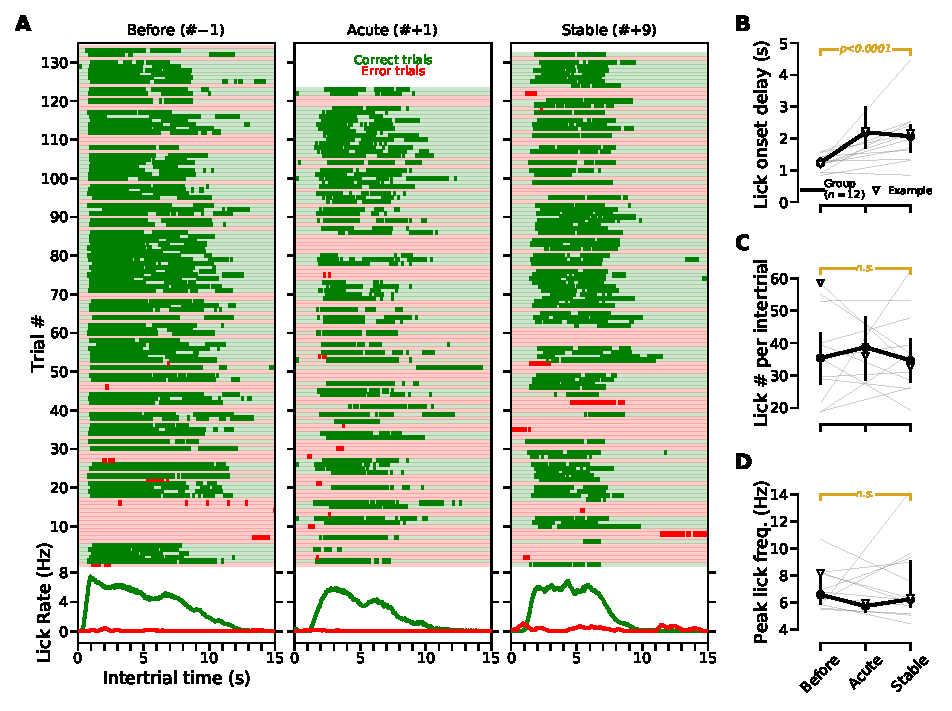
\includegraphics[width=\textwidth]{ch-lesion/figures/Lick.pdf}
        \caption[Licking Behavior After Striatal Lesion]
        {\textbf{Licking behavior after dS lesion.}
        \textbf{A)} Trial-by-trial licking pattern (\textit{top}) and averaged lick rate aligned to intertrial onset for a single animal in 3 sessions (1 just before and 2 after lesion).
        \textbf{B-D)} Effect of striatal lesion on lick onset delay (\textbf{B}), number of licks per intertrial (\textbf{C}) and peak lick frequency (\textbf{D})
        Same color code for individual lesion type as in \autoref{fig:lesion:task}.
        }
        \label{fig:lesion:lick}
    \end{center}
\end{figure}